\documentclass{article}
\usepackage{pgfplots, amssymb, amsmath, darkmode, fullpage, tikz,array }
\usepackage{tcolorbox}
\usetikzlibrary{shapes.geometric, arrows}
\usetikzlibrary{positioning}

\tikzstyle{startstop} = [square/.style={regular polygon,regular polygon sides=4}, rounded corners, minimum width=3cm, minimum height=1cm,text centered, draw=black, fill=red!20]
\tikzstyle{process} = [rectangle, minimum width=1cm, minimum height=1cm, text centered, draw=black]
\tikzstyle{io} = [trapezium, trapezium left angle=70, trapezium right angle=110, minimum width=0.5cm, minimum height=0.5cm, text centered, draw=black, fill=green!20]

\tikzstyle{arrow} = [thick,->,>=stealth]

\begin{document}
\begin{center}
    \section{Parallelization}    
    \end{center}
    
    \begin{sloppypar}
        \indent{} In the grand scheme of calculations, there comes a point when there is a limiting factor in which the amount of operations per second becomes an inhibitor. As previously mentioned, the Discrete Fourier Transform has time complexity of $O(N^2)$, where $N$ is the vector size (for an $NxN$ matrix this expands to: $O(N^2N^2) = O(N^4)$). In contrast, the Fast Fourier Transform has time complexity of $O(Nlog(N))$ ($O(N^2log(N))$ when expanded to $NxN$).
    \end{sloppypar}
    \vspace{2mm}
    \begin{center}
        %don't ask me how this worked it just did
    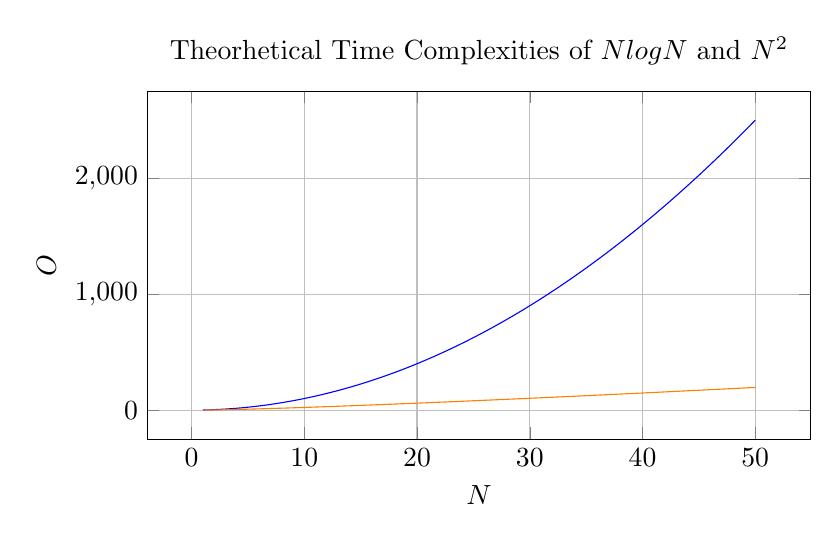
\begin{tikzpicture}
            \begin{axis}[
                xlabel={$N$},
                ylabel={$O$},
                title={Theorhetical Time Complexities of $NlogN$ and $N^2$},
                grid=major,
                width=10cm,
                height=6cm,
                domain=1:50,
                samples=5000,
            ]
                \addplot[color=blue]{x^2};
                \addplot[color=orange]{x*ln(x)};
            \end{axis}
    \end{tikzpicture}
    \end{center}
    \begin{sloppypar}
        \indent{}In computers there are two major processing units: Graphics processing unit and Central processing Unit. The CPU is made with a handful of cores while a modern GPU has thousands. Different processes can be offloaded to each core.
        This is where the time complexity of $O(nlogn)$ makes this so good for modern computers. We can offload the 'split' vectors/matrices to different GPU cores and compute each of these piecewise. Figure 2 below shows a rudimentary theorhetical graph of what this would look like. 
    \end{sloppypar}
    %I Hate this Figure
    \begin{figure}[h]
    \centering
    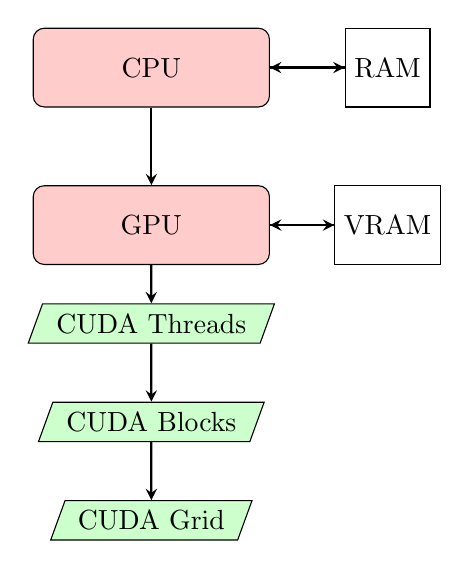
\begin{tikzpicture}
        %graph threads or IO
        \node (CPU) [startstop] {CPU};
        \node (RAM) [process, right of=CPU, xshift=2cm] {RAM};
        \node (GPU) [startstop, below of=CPU, yshift=-1cm] {GPU};
        \node (VRAM)[process, right of=GPU, xshift=2cm] {VRAM};
        \node (Threads)[io, below of=GPU, yshift=-0.25cm] {CUDA Threads};
        \node (Blocks) [io, below of=Threads, yshift=-0.25cm] {CUDA Blocks};
        \node (Grid) [io, below of=Blocks, yshift=-0.25cm] {CUDA Grid};
        %technically should flip from Grid ->Blocks->threads since its instantiated in a Kernel then the Kernel throws it to a grid if applicable
        %arrows
        \draw [arrow] (CPU) -- (RAM);
        \draw [arrow] (RAM) -- (CPU);
        \draw [arrow] (CPU) -- (GPU);
        \draw [arrow] (GPU) -- (VRAM);
        \draw [arrow] (VRAM) -- (GPU);
        \draw [arrow] (GPU) -- (Threads);
        \draw [arrow] (Threads) -- (Blocks);
        \draw [arrow] (Blocks) -- (Grid);
    \end{tikzpicture}
        \caption{CUDA GPU Parallelization for FFT}
    \end{figure}
    \begin{sloppypar}
        \indent{}To demysitfy this graph, one must first understand that it is not possible to know \emph{exactly} what is happening on any set core. CUDA grids are collections of CUDA Blocks and CUDA Blocks are collections of CUDA Threads. CUDA Threads
        are the pieces of information that work on some part of the FFT. This can be doing the actual calculations, the combinations, or putting it into a new vector. If the tasks are similar enough they will get diverted to a CUDA Block. A CUDA Block is a collection of these threads. So this is 
        using the VRAM over threads to share and seperately compute information. The Block works on something called a streaming multiprocessor. This is a collection of CUDA cores on a shared piece of L1,L2 Cache (on processor memory) or VRAM. If the process stream is big enough, multiple Blocks can be executed.
        This is called a CUDA Grid. A single streaming multiprocessor is only capable of working on Blocks. A CUDA Grid will take multiple streaming multiprocessors are use them to work on the same area of calculations, but divert tasks to Blocks. 
    \end{sloppypar}
    \begin{sloppypar}
        \indent{} The new question is now how can we look at the FFT and Matlab's utilization of CUDA parallel processing to get a better understanding of why it is more effcient.
    \end{sloppypar}
\end{document}